%%%%%%%%%%%%%%%%%%%%%%%%%%%%%%%%%%%%%%
%%%%%%%%%%%%%%%%%%%%%%%%%%%%%%%%%%%%%%
% Do not edit the TeX file your work
% will be overwritten.  Edit the RnW
% file instead.
%%%%%%%%%%%%%%%%%%%%%%%%%%%%%%%%%%%%%%
%%%%%%%%%%%%%%%%%%%%%%%%%%%%%%%%%%%%%%





\newcommand{\DefineMacros}{
\newcommand{\AlexNSur}{4,364}
\newcommand{\AlexNTar}{4,085,282}
\newcommand{\AlexSurmean}{0.462}
\newcommand{\AlexMrp}{0.288}
\newcommand{\AlexMrpSD}{0.0169}
\newcommand{\AlexRaking}{0.263}
\newcommand{\AlexRefitTimeHours}{10}
\newcommand{\AlexMrPawTimeSecs}{16}
\newcommand{\LaxNSur}{6,341}
\newcommand{\LaxNTar}{9,694,541}
\newcommand{\LaxSurmean}{0.333}
\newcommand{\LaxMrp}{0.337}
\newcommand{\LaxMrpSD}{0.039}
\newcommand{\LaxRaking}{0.33}
\newcommand{\LaxRefitTimeHours}{11}
\newcommand{\LaxMrPawTimeSecs}{23}

}


% Define the graph lists





%%%%%%%%%%%%%%%%%%%%%%
% Plots


\newcommand{\WeightPlot}{

\begin{knitrout}
\definecolor{shadecolor}{rgb}{0.969, 0.969, 0.969}\color{fgcolor}\begin{figure}[!h]

{\centering 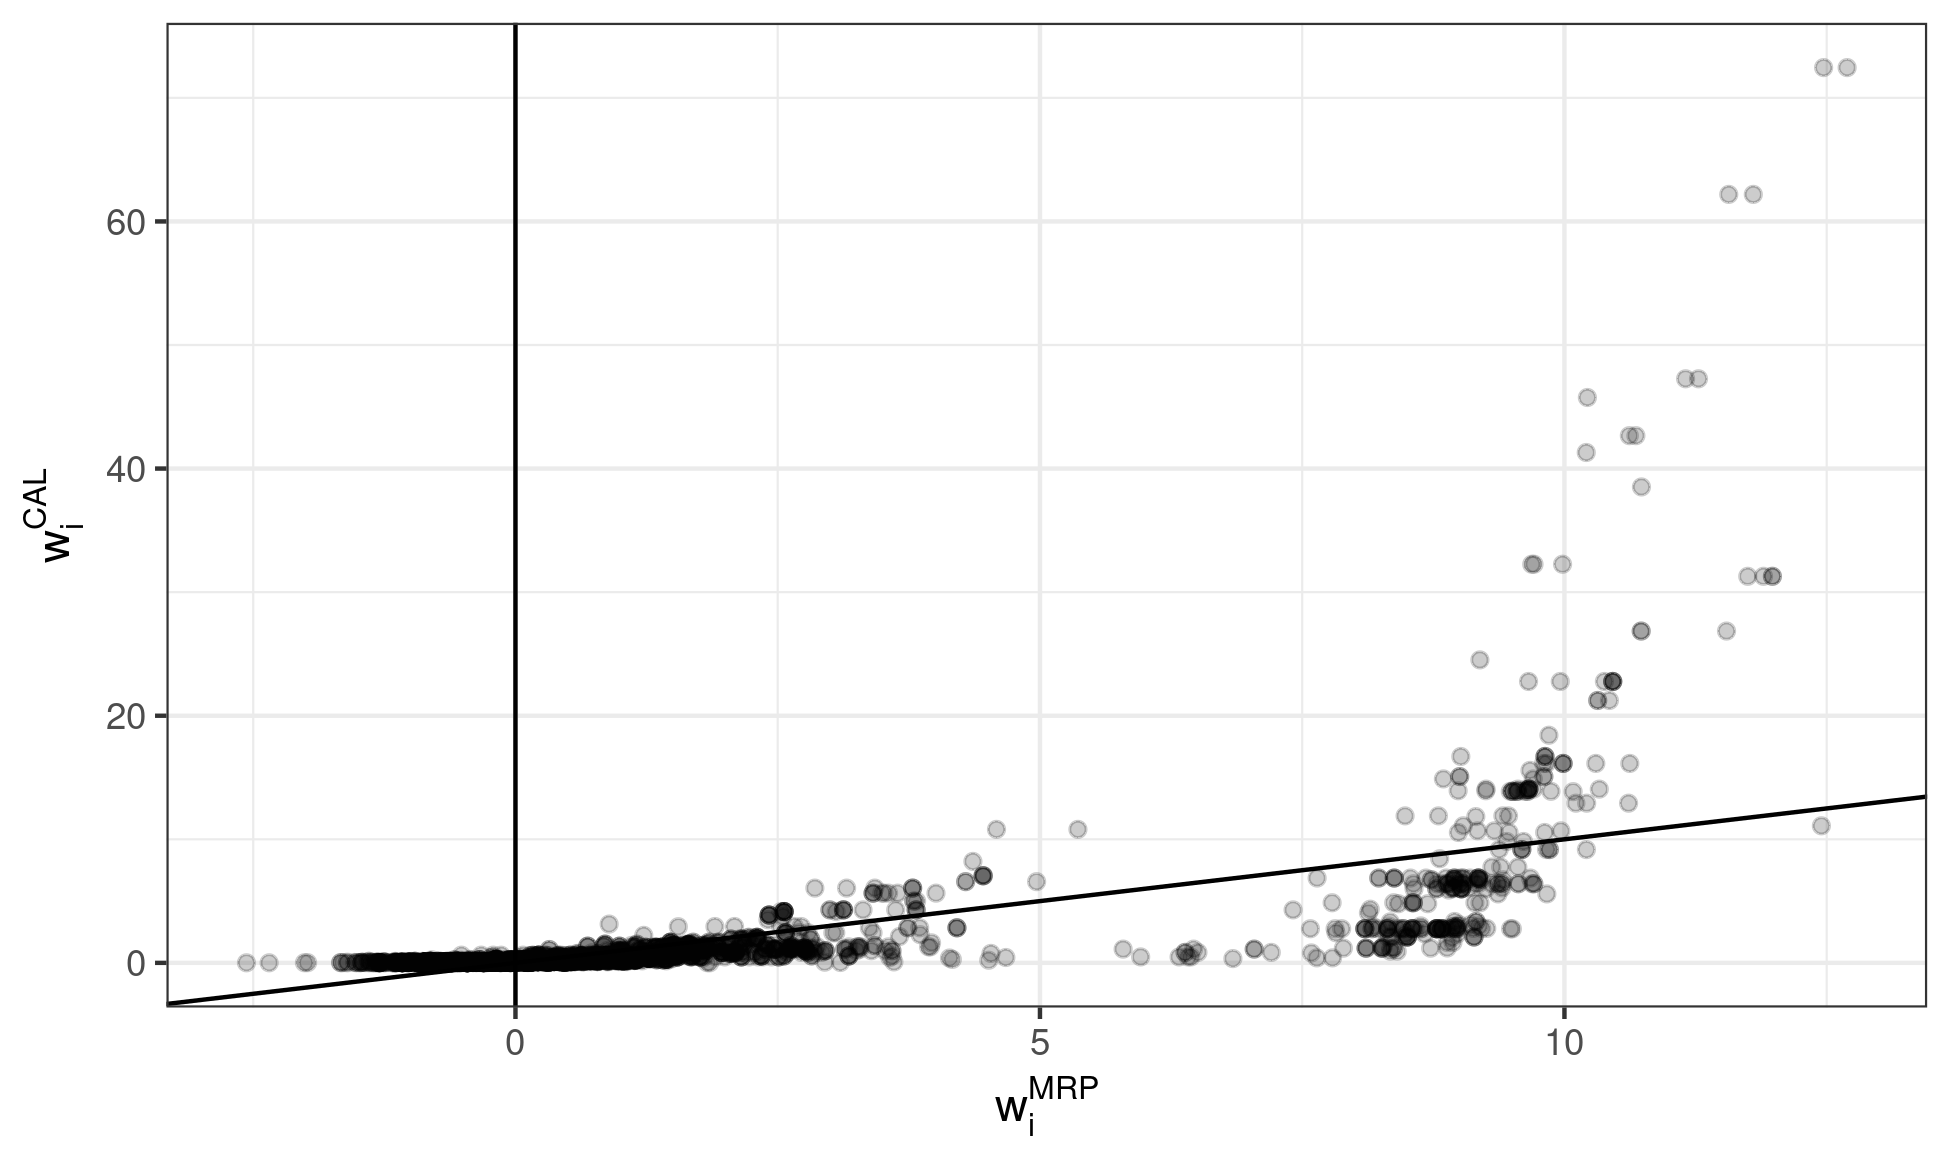
\includegraphics[width=0.98\linewidth,height=0.588\linewidth]{figure/weightplot-1} 

}

\caption[Comparison between raking and MrPlew weights for a particular example]{Comparison between raking and MrPlew weights for a particular example}\label{fig:weightplot}
\end{figure}

\end{knitrout}
}


\newcommand{\AlexanderImbalancePrimary}{

\begin{knitrout}
\definecolor{shadecolor}{rgb}{0.969, 0.969, 0.969}\color{fgcolor}\begin{figure}[!h]

{\centering 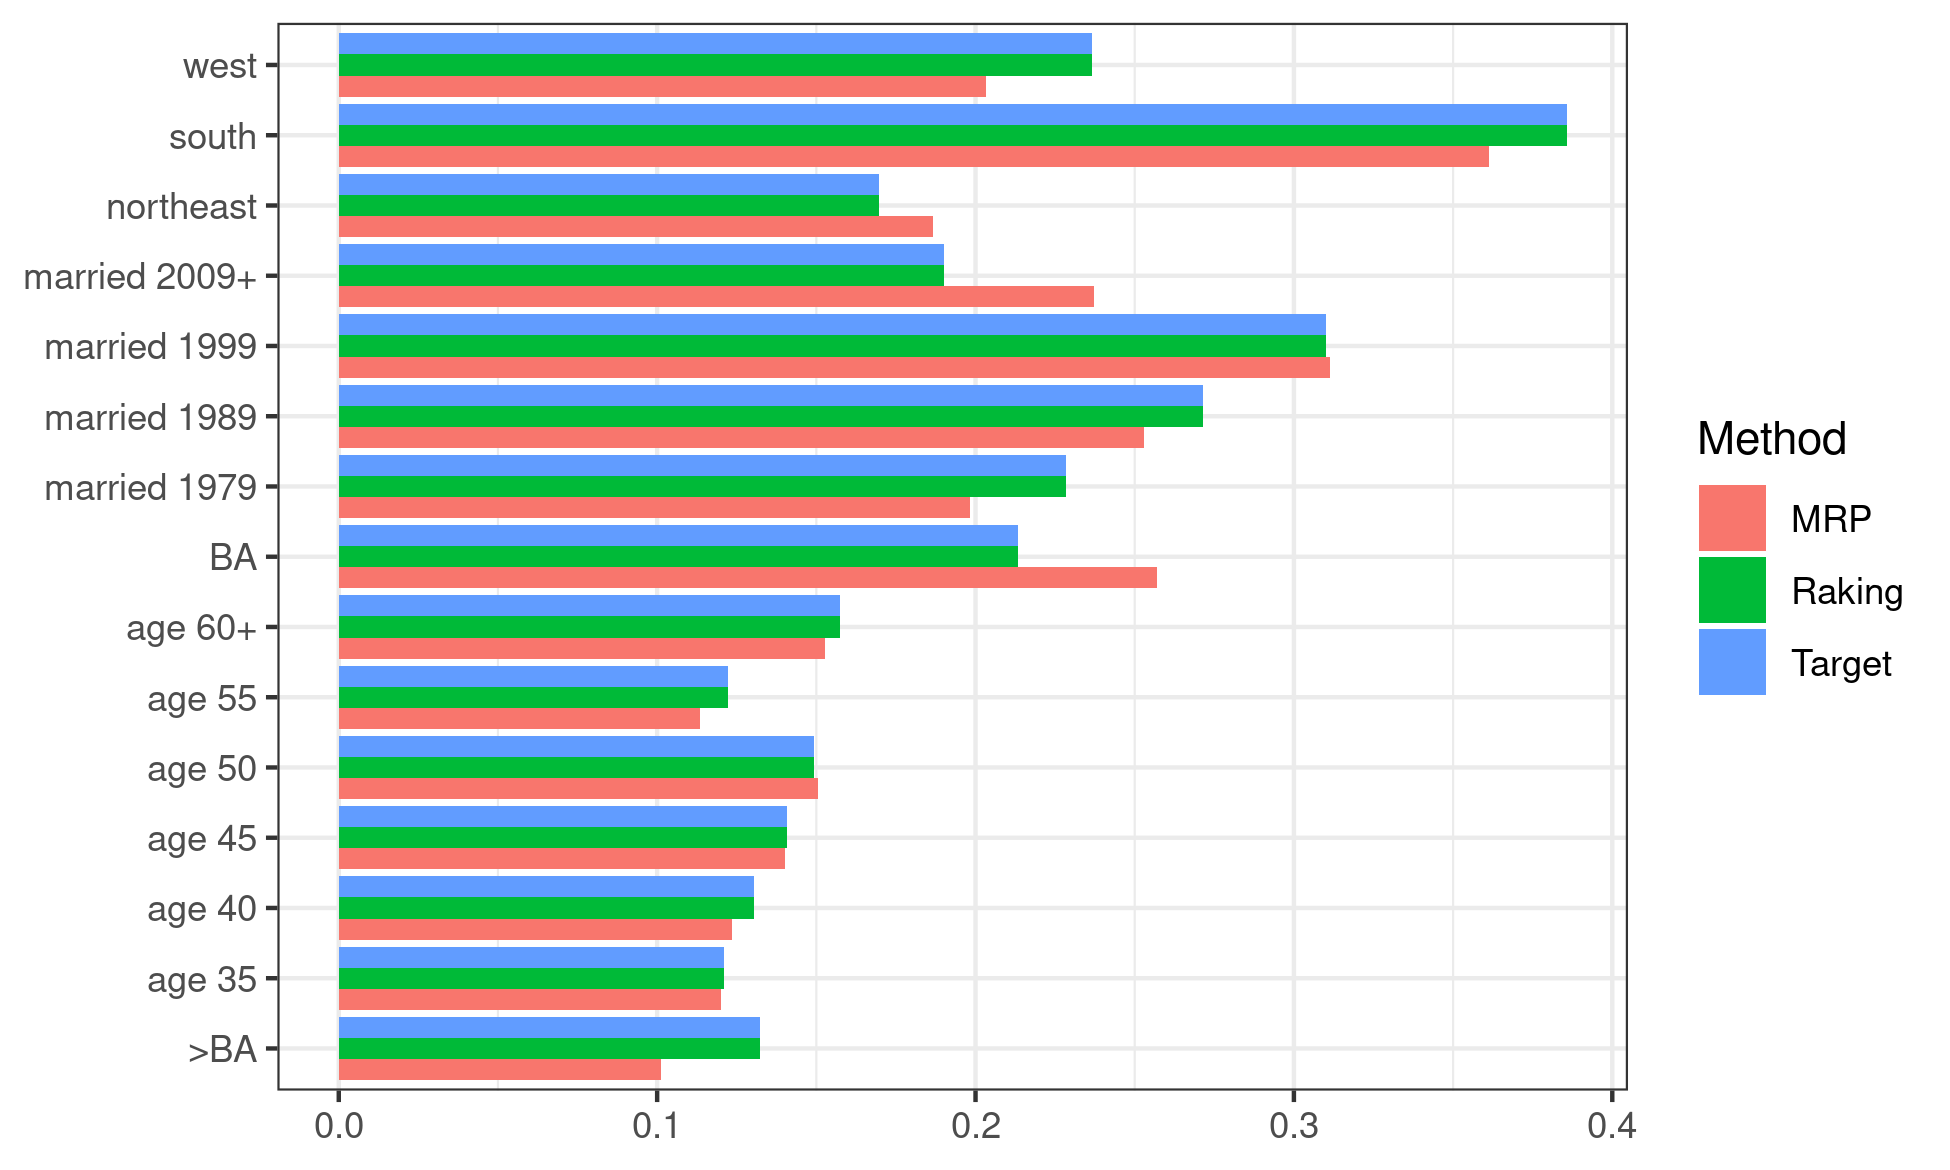
\includegraphics[width=0.98\linewidth,height=0.588\linewidth]{figure/alexanderprimary-1} 

}

\caption[Imbalance plot for primary effects]{Imbalance plot for primary effects}\label{fig:alexanderprimary}
\end{figure}

\end{knitrout}
}


\newcommand{\AlexanderImbalanceInteraction}{

\begin{knitrout}
\definecolor{shadecolor}{rgb}{0.969, 0.969, 0.969}\color{fgcolor}\begin{figure}[!h]

{\centering 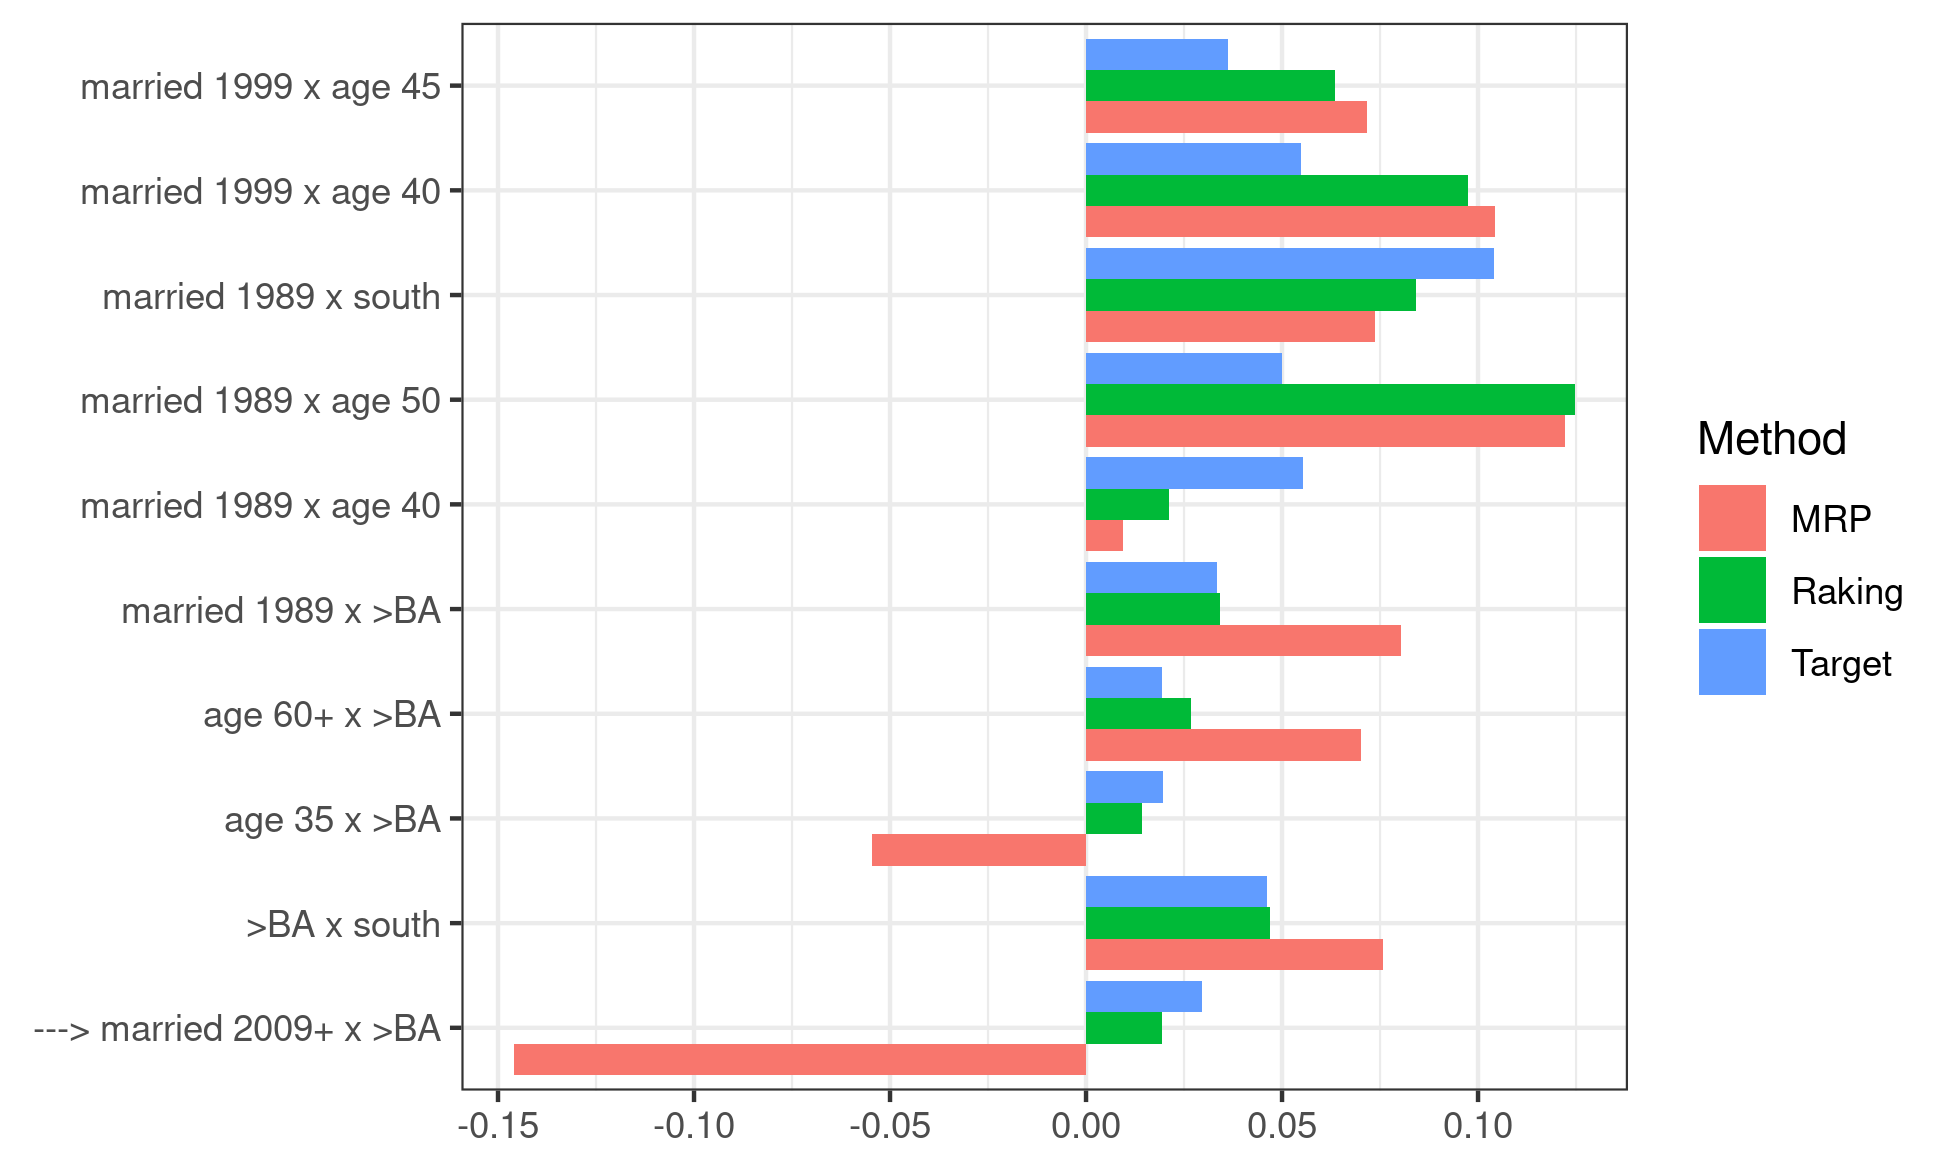
\includegraphics[width=0.98\linewidth,height=0.588\linewidth]{figure/alexanderinteraction-1} 

}

\caption[Imbalance plot for select interaction effects]{Imbalance plot for select interaction effects}\label{fig:alexanderinteraction}
\end{figure}

\end{knitrout}
}




\newcommand{\AlexanderPredictionFigOne}{

\begin{knitrout}
\definecolor{shadecolor}{rgb}{0.969, 0.969, 0.969}\color{fgcolor}\begin{figure}[!h]

{\centering 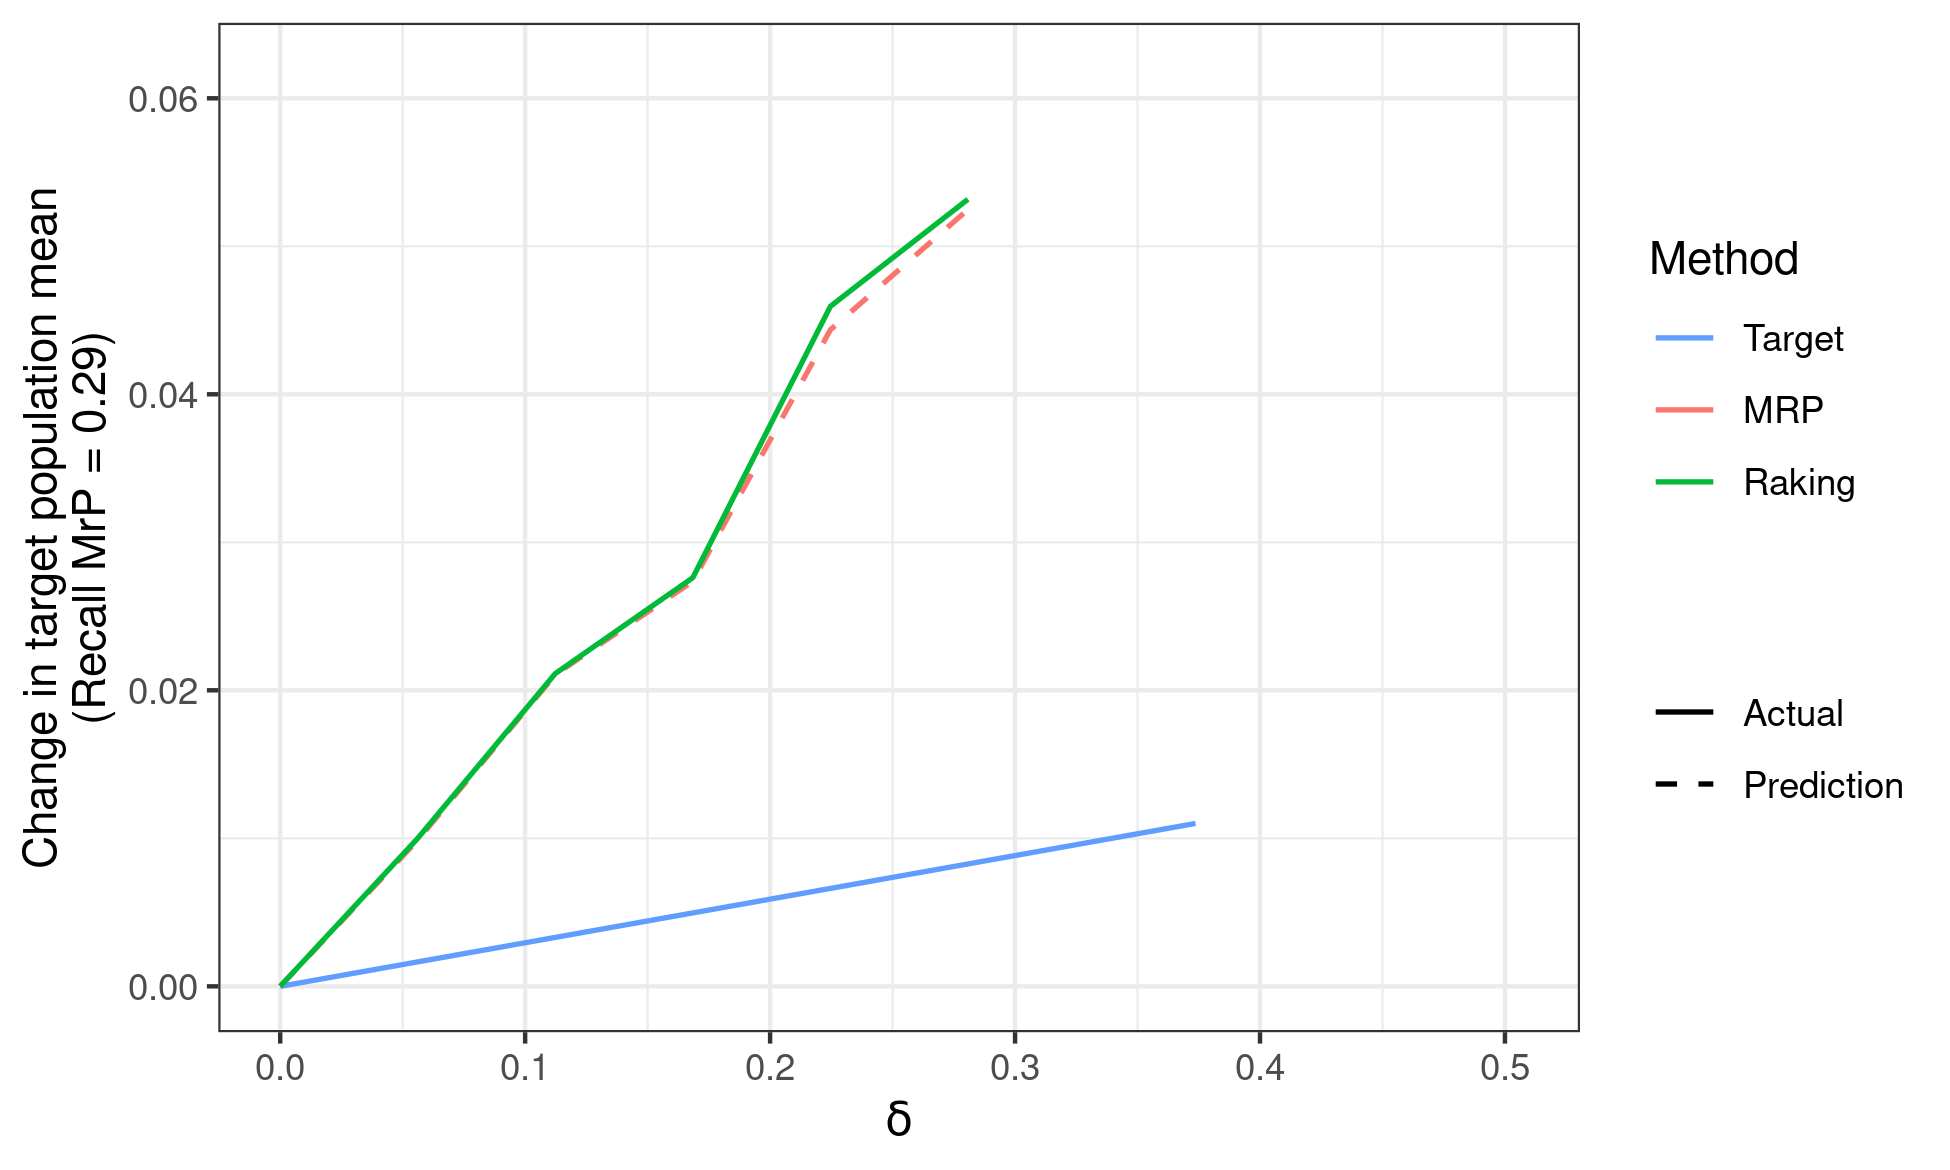
\includegraphics[width=0.98\linewidth,height=0.588\linewidth]{figure/alexandercontpred-1} 

}

\caption[Predictions for the name change dataset]{Predictions for the name change dataset}\label{fig:alexandercontpred}
\end{figure}

\end{knitrout}
}



\newcommand{\AlexanderPredictionFigTwo}{

\begin{knitrout}
\definecolor{shadecolor}{rgb}{0.969, 0.969, 0.969}\color{fgcolor}\begin{figure}[!h]

{\centering 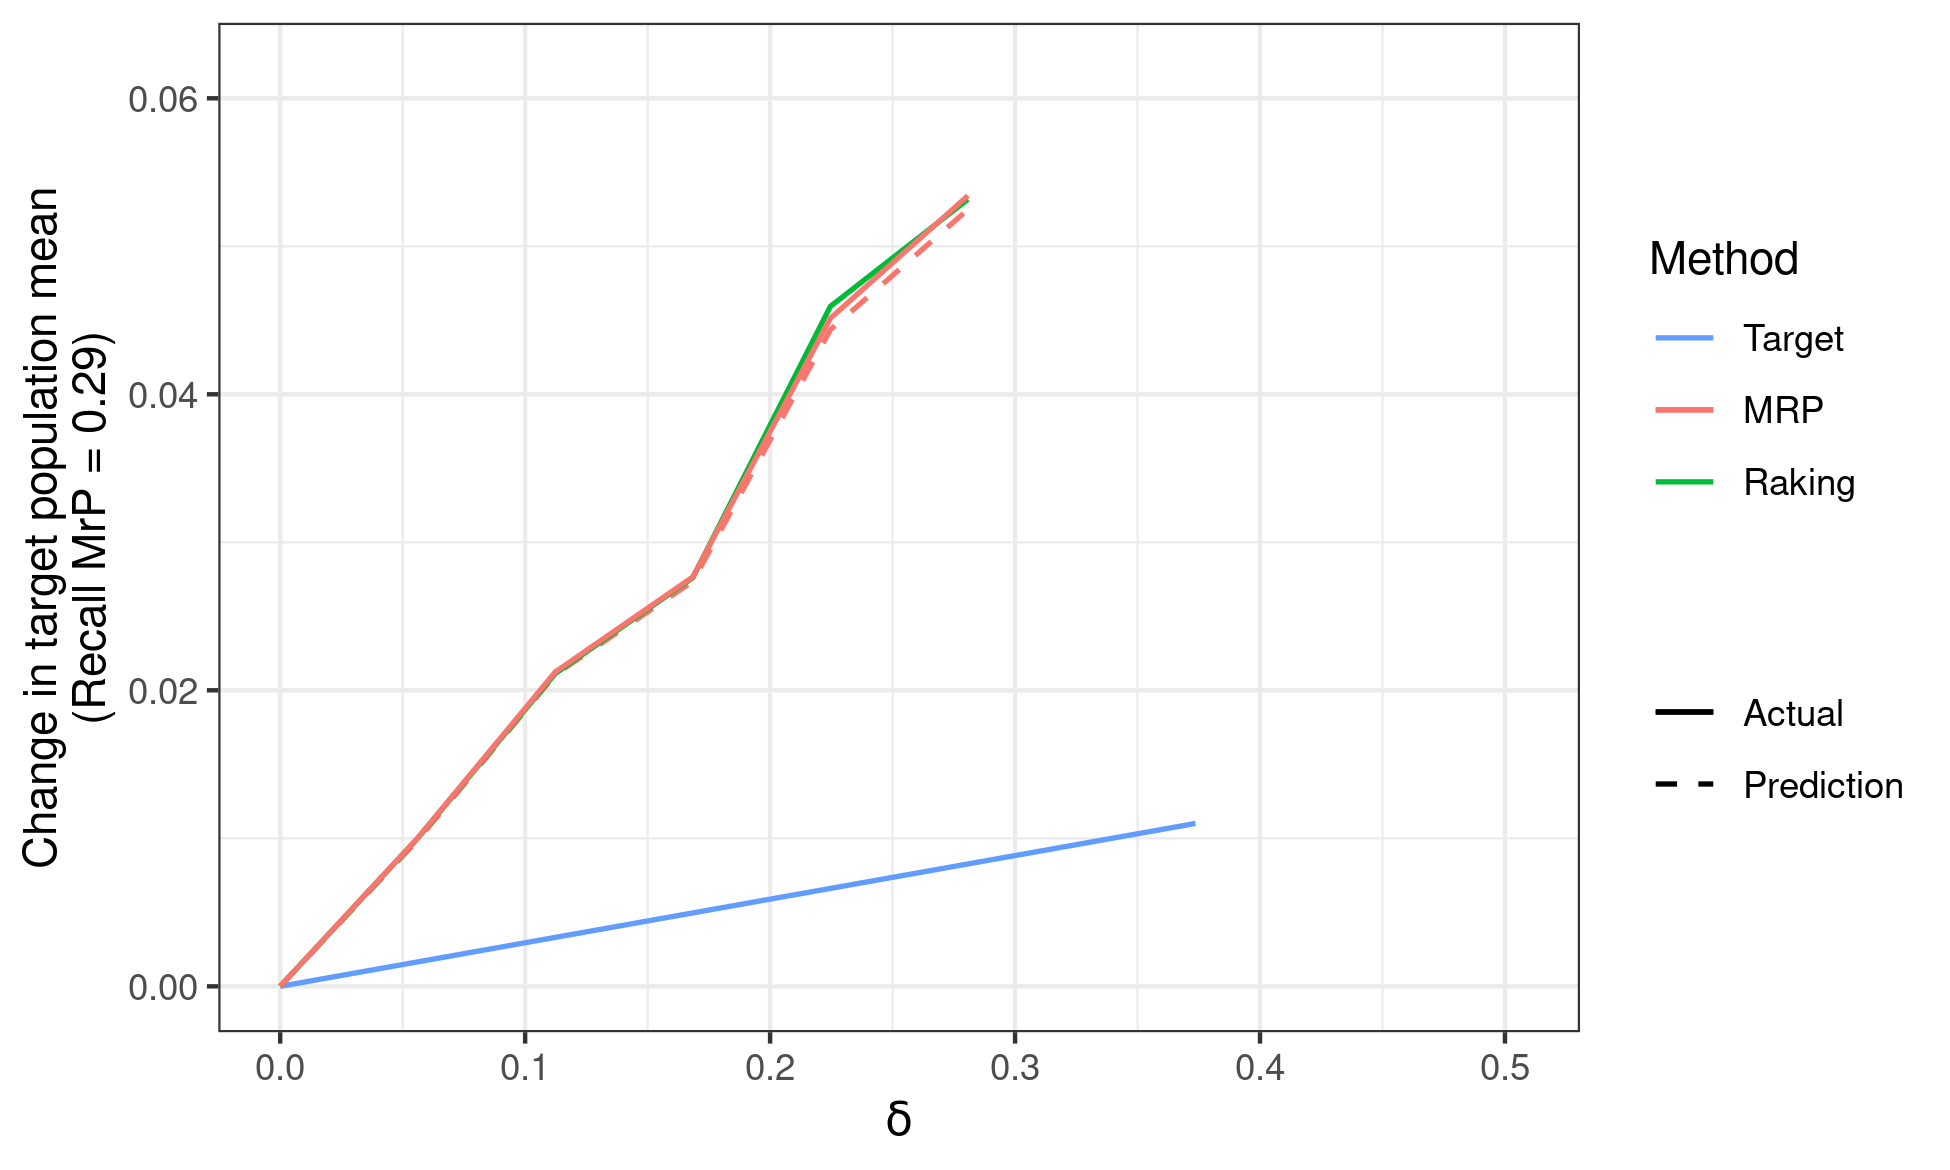
\includegraphics[width=0.98\linewidth,height=0.588\linewidth]{figure/alexanderdiscretepred-1} 

}

\caption[Predictions and refit for the name change dataset]{Predictions and refit for the name change dataset}\label{fig:alexanderdiscretepred}
\end{figure}

\end{knitrout}
}



% \newcommand{\AlexanderPredictionFigThree}{
% <<>>=
% figcap <- paste0("Continuous predictions Alexander")
% @
% <<alexanderbinarypred, cache=cache, fig.show='hold', fig.cap=figcap>>=
% print(pred_plot_3)
% @
% }




% \newcommand{\AlexanderPredictionFigFour}{
% <<>>=
% figcap <- paste0("Continuous predictions Alexander")
% @
% <<alexanderrefit, cache=cache, fig.show='hold', fig.cap=figcap>>=
% print(pred_plot_4)
% @
% }
